
\section{Simulated Data and Event Weighting}

After formulating our problem as a supervised learning task, the next step is to find an appropriate way to tackle it.
To train a classifier, we need a set of labeled observations. In the context of particle physics, each observation is an
event and the label corresponds to the process that led to this event. However, obtaining these labeled observations is
not as straightforward as simply recording the events.

We need a model that describes the underlying physics. In our case, this is the \gls{sm}, including the branching
factors introduced before. The model is based on our understanding of particle physics and describes the probabilities
of different processes and outcomes.

To generate our labeled dataset, we use a tool called \gls{mc} simulations. \gls{mc} simulations are a way to generate
data that follows a given model. In essence, the simulation creates a large number of events, each following the
probabilistic rules of the model. We can then record these events and their corresponding labels (which process they
were created by).

The benefit of \gls{mc} simulations is that they allow us to create a large amount of data where we know the 'true' labels.
This data can be used to train and evaluate our classifier. However, it's important to note that while \gls{mc} simulations
are based on our best understanding of physics, they are not perfect. There are always uncertainties and potential
inaccuracies in the model, which can affect the generated data and the performance of our classifier.

To alleviate the difficulties of training on small dataset, more signal events are explicitly generated. This leads to
producing a different distribution than the one observed in the real data. To align the \gls{mc} simulated data with the real
data, it is necessary to apply event weights. Event weighting is a technique used to correct the simulated distributions
for known differences between the simulation and the real data.

% Event weights can account for a variety of effects:

% Luminosity: The total number of simulated events often does not correspond to the luminosity of the real data. Events
% are therefore weighted to correspond to the correct integrated luminosity. If $L_{data}$ is the integrated luminosity of
% the data and $L_{\gls{mc}}$ is the integrated luminosity of the \gls{mc} sample, then the luminosity weight for an event is $w_{L} =
%     L_{data}/L_{\gls{mc}}$.

% Cross-Section: Different processes have different probabilities (cross-sections) of occurring. The ratio of the
% cross-sections in data and simulation $\sigma_{data}/\sigma_{\gls{mc}}$ is used as a weight.

% Detector Effects: The detector response is not always perfectly simulated. Therefore, weights are applied to correct for
% known discrepancies in detector efficiencies and energy resolutions between the data and the simulation.

% Pileup: Pileup refers to additional proton-proton collisions that occur simultaneously with the event of interest.
% Pileup can significantly affect the event reconstruction. Pileup weights are used to match the pileup distribution in
% the data.

% Higher-order corrections: Theoretical predictions often include higher-order corrections, known as K-factors, to account
% for processes beyond the leading-order approximation used in the simulation.

% In mathematical terms, the total weight $w_{total}$ for an event can be written as the product of individual weights:

% \begin{equation}
%     w_{\text{total}} = w_{L} w_{\sigma} w_{\text{detector}} w_{\text{pileup}} w_{\text{K-factor}}
% \end{equation}

% Event weights are essential for ensuring that the simulated events accurately represent the conditions of the actual
% experiment. These weights allow us to make meaningful comparisons between the data and theoretical predictions, and are
% a crucial part of the analysis in high-energy physics.


% \section{V8 adaptation}

\section{\gls{sr} cut expression}
\label{appendix:cut-expression}

{\scriptsize
    \begin{verbatim}
    custTrigMatch_LooseID_FCLooseIso_DLT
    && (dilep_type && (lep_ID_0*lep_ID_1)>0)
    && ((lep_Pt_0 >= 10e3 && lep_Pt_1 >= 10e3) && (fabs(lep_Eta_0) <= 2.5 && fabs(lep_Eta_1) <= 2.5)
        && ((abs(lep_ID_0) == 13 && lep_isMedium_0 && lep_isolationLoose_VarRad_0 && passPLIVTight_0)
            || ((abs(lep_ID_0) == 11 && lep_isTightLH_0 && lep_isolationLoose_VarRad_0 && passPLIVTight_0
                && lep_ambiguityType_0 == 0 && lep_chargeIDBDTResult_recalc_rel207_tight_0 > 0.7)
                && ((!(!(lep_Mtrktrk_atConvV_CO_0 < 0.1 && lep_Mtrktrk_atConvV_CO_0 >= 0 && lep_RadiusCO_0 > 20)
                    && (lep_Mtrktrk_atPV_CO_0 < 0.1 && lep_Mtrktrk_atPV_CO_0 >= 0)))
                    && !(lep_Mtrktrk_atConvV_CO_0 <0.1 && lep_Mtrktrk_atConvV_CO_0 >= 0 && lep_RadiusCO_0 > 20))))
            && ((abs(lep_ID_1) == 13 && lep_isMedium_1 && lep_isolationLoose_VarRad_1 && passPLIVTight_1)
                || ((abs(lep_ID_1) == 11 && lep_isTightLH_1 && lep_isolationLoose_VarRad_1 && passPLIVTight_1
                    && lep_ambiguityType_1 == 0 && lep_chargeIDBDTResult_recalc_rel207_tight_1 > 0.7)
                    && ((!(!(lep_Mtrktrk_atConvV_CO_1 < 0.1 && lep_Mtrktrk_atConvV_CO_1 >= 0 && lep_RadiusCO_1 > 20)
                        && (lep_Mtrktrk_atPV_CO_1 < 0.1 && lep_Mtrktrk_atPV_CO_1 >= 0)))
                        && !(lep_Mtrktrk_atConvV_CO_1 < 0.1 && lep_Mtrktrk_atConvV_CO_1 >= 0 && lep_RadiusCO_1 > 20)))))
    && nTaus_OR==1
    && nJets_OR_DL1r_85>=1
    && nJets_OR>=4
    && ((dilep_type==2) || abs(Mll01-91.2e3)>10e3)
\end{verbatim}
}

We have kept the cuts the same as \cite{severin}, except for the cut on the \verb|nJets_OR| to \verb|>=4| to keep
consistent definition \gls{sr} definition across the group \todo{refer to the BDT group - how?}.

\section{Yields Plots}
\label{appendix:yields}

\begin{figure}[htb!]
    \centering
    \begin{subfigure}{0.45\textwidth}
        \includegraphics[width=\linewidth]{figures/yields/lep-pt-0.pdf}
        \caption{Distribution of the transverse momentum of the leading lepton.}
    \end{subfigure}\hfill%
    \begin{subfigure}{0.45\textwidth}
        \includegraphics[width=\linewidth]{figures/yields/lep-pt-1.pdf}
        \caption{Distribution of the transverse momentum of the subleading lepton.}
    \end{subfigure}
\end{figure}

\begin{figure}[htb!]
    \centering
    \begin{subfigure}{0.45\textwidth}
        \includegraphics[width=\linewidth]{figures/yields/n-jets.pdf}
        \caption{Distribution of the number of jets.}
    \end{subfigure}\hfill%
    \begin{subfigure}{0.45\textwidth}
        \includegraphics[width=\linewidth]{figures/yields/n-bjets.pdf}
        \caption{Distribution of the number of $b$-jets.}
    \end{subfigure}
\end{figure}

\begin{figure}[htb!]
    \centering
    \begin{subfigure}{0.45\textwidth}
        \includegraphics[width=\linewidth]{figures/yields/tau-width.pdf}
        \caption{Distribution of the $\tau$-jet width.}
    \end{subfigure}\hfill%
\end{figure}
\subsection{List of samples by each process}

The root directory for the files is:

{\small
\verb|/eos/atlas/atlascerngroupdisk/phys-higgs/HSG8/multilepton_ttWttH/v08/v0801/systematics-full/nominal|
}

The list of samples is given in \hyperref[tab:samples]{Table~\ref*{tab:samples}}.

\newpage

\begin{table}[h!]
    \centering
    \renewcommand{\arraystretch}{1.5}
    \caption{List of samples by each process}
    \label{tab:samples}
    \begin{tabular}{p{1.5cm}p{13.5cm}}
        \toprule
        Process      & \gls{dsid}                                                           \\
        \midrule
        $t\bar{t}H$  & p4498/346343, p4498/346344, p4498/346345                             \\
        $t\bar{t}W$  & p4416/700168, p4590/700205                                           \\
        $t\bar{t}Z$  & p4416/700168                                                         \\
        $t\bar{t}$   & p4308/410470                                                         \\
        $VV$         & p4416/364250, p4416/364253, p4416/364254, p4416/364255, p4308/364283, p4308/364284, p4308/364285,
p4308/364286, p4308/364287, p4308/363355, p4308/363356, p4308/363357, p4308/363358, p4308/363359,
p4308/363360, p4308/363489                                               \\
        $ggVV$       & p4308/345705, p4396/345706, p4396/345715, p4396/345718, p4396/345723 \\
        $Zjets$      & p4308/364100, p4308/364101, p4308/364102, p4308/364103, p4308/364104, p4308/364105, p4308/364106,
p4308/364107, p4308/364108, p4308/364109, p4308/364110, p4308/364111, p4308/364112, p4308/364113,
p4308/364114, p4308/364115, p4308/364116, p4308/364117, p4308/364118, p4308/364119, p4308/364120,
p4308/364121, p4308/364122, p4308/364123, p4308/364124, p4308/364125, p4308/364126, p4308/364127,
p4308/364128, p4308/364129, p4308/364130, p4308/364131, p4308/364132, p4308/364133, p4308/364134,
p4308/364135, p4308/364136, p4308/364137, p4308/364138, p4308/364139, p4308/364140, p4308/364141,
p4308/364198, p4308/364199, p4308/364200, p4308/364201, p4308/364202, p4308/364203, p4308/364204,
p4308/364205, p4308/364206, p4308/364207, p4308/364208, p4308/364209, p4308/364210, p4308/364211,
p4308/364212, p4308/364213, p4308/364214, p4308/364215                                            \\
        $Wjets$      & p4308/364156, p4308/364157, p4308/364158, p4308/364159, p4308/364160, p4308/364161, p4308/364162,
p4308/364163, p4308/364164, p4308/364165, p4308/364166, p4308/364167, p4308/364168, p4308/364169,
p4308/364170, p4308/364171, p4308/364172, p4308/364173, p4308/364174, p4308/364175, p4308/364176,
p4308/364177, p4308/364178, p4308/364179, p4308/364180, p4308/364181, p4308/364182, p4308/364183,
p4308/364184, p4308/364185, p4308/364186, p4308/364187, p4308/364188, p4308/364189, p4308/364190,
p4308/364191, p4308/364192, p4308/364193, p4308/364194, p4308/364195, p4308/364196, p4308/364197                                            \\
        $tW$         & p4308/410646, p4308/410647                                           \\
        $threeTop$   & p4308/304014                                                         \\
        $fourTop$    & p4308/410080                                                         \\
        $t\bar{t}WW$ & p4308/410081                                                         \\
        $tZ$         & p4308/410560                                                         \\
        $WtZ$        & p4308/410408                                                         \\
        $VVV$        & p4308/364242, p4308/364243, p4308/364244, p4308/364245, p4308/364246, p4308/364247, p4308/364248, p4308/364249                                              \\
        $VH$         & p4308/342284, p4308/342285                                           \\
        $tHjb$       & p4308/346799\_AF                                                     \\
        $tWH$        & p4308/346678\_AF                                                     \\
        \bottomrule
    \end{tabular}
\end{table}

\newpage
\subsection{Distribution of the variables inside \gls{sr}}

The following figures (\autoref{fig:distributions1} and \autoref{fig:distributions2}) show the distributions of some variables
of interest inside \gls{sr}.

\captionsetup[subfigure]{justification=centering}
\begin{figure}[htb!]
    \centering
    \begin{subfigure}{0.45\textwidth}
        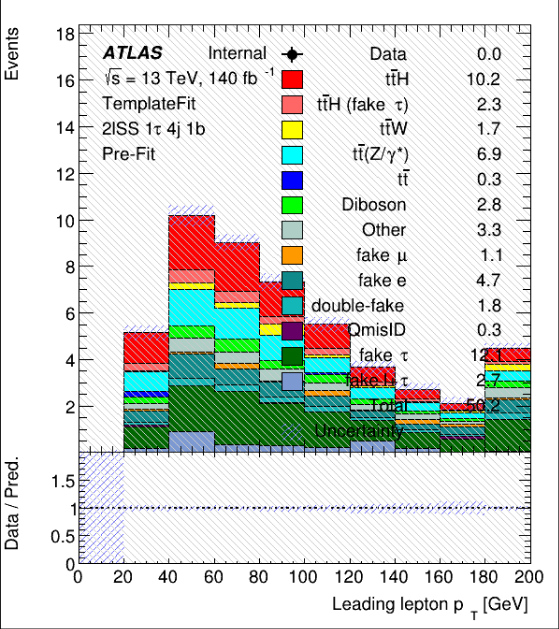
\includegraphics[width=\linewidth]{figures/plots/histograms/lep_pt_0.png}
        \caption{Distribution of the transverse momentum of the leading lepton.}
        \label{fig:lep_pt_0}
    \end{subfigure}\hfill%
    \begin{subfigure}{0.45\textwidth}
        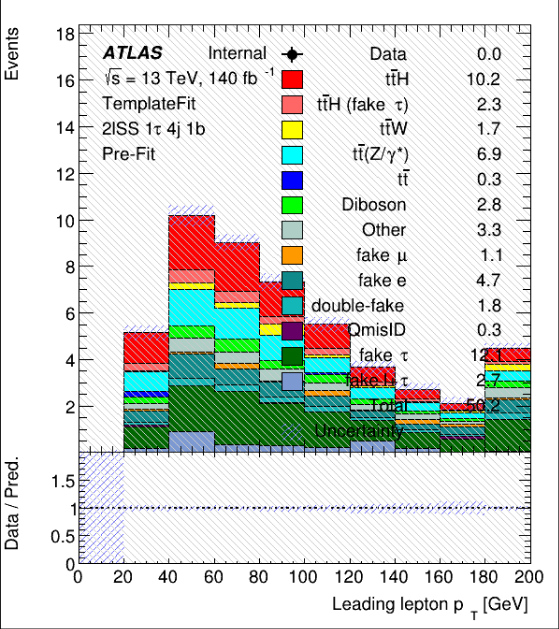
\includegraphics[width=\linewidth]{figures/plots/histograms/lep_pt_1.png}
        \caption{Distribution of the transverse momentum of the subleading lepton.}
        \label{fig:lep_pt_1}
    \end{subfigure}

    \vspace{0.5cm}

    \begin{subfigure}{0.45\textwidth}
        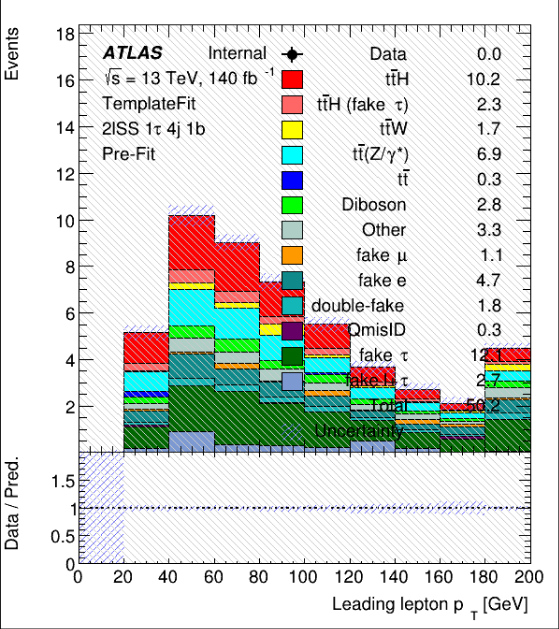
\includegraphics[width=\linewidth]{figures/plots/histograms/lep_Eta_0.png}
        \caption{Distribution of the pseudorapidity of the leading lepton.}
        \label{fig:lep_Eta_0}
    \end{subfigure}\hfill%
    \begin{subfigure}{0.45\textwidth}
        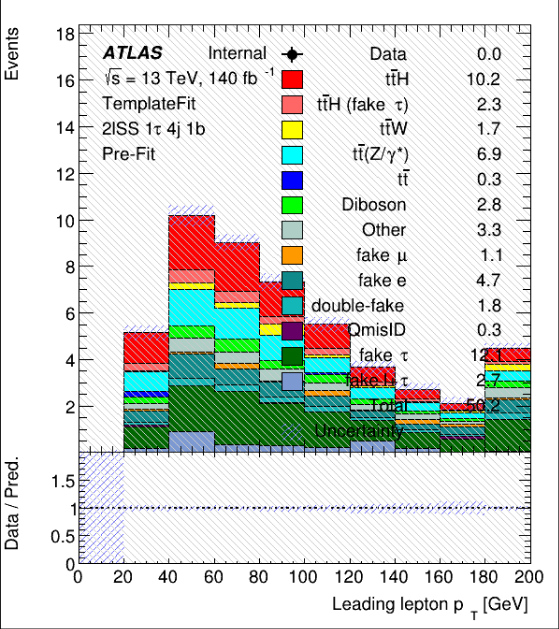
\includegraphics[width=\linewidth]{figures/plots/histograms/lep_Eta_1.png}
        \caption{Distribution of the pseudorapidity of the subleading lepton.}
        \label{fig:lep_Eta_1}
    \end{subfigure}
    \caption{Distributions of the variables inside \gls{sr} (part 1)}
    \label{fig:distributions1}
\end{figure}

\newpage

\begin{figure}[htb!]
    \centering
    \begin{subfigure}{0.45\textwidth}
        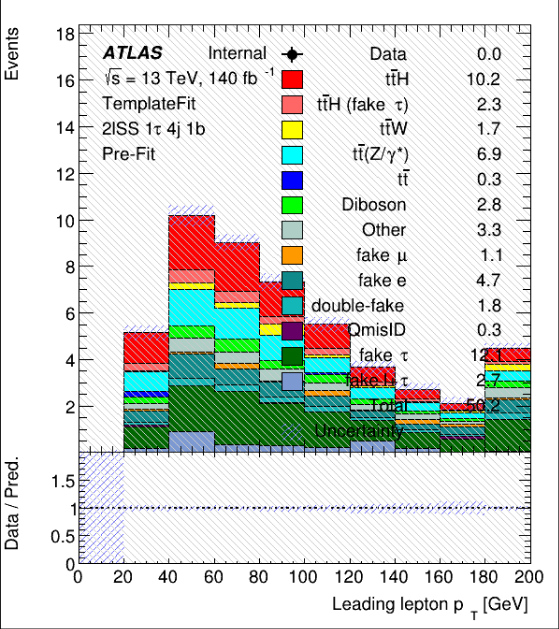
\includegraphics[width=\linewidth]{figures/plots/histograms/lep_Phi_0.png}
        \caption{Distribution of the azimuthal angle of the leading lepton.}
        \label{fig:lep_Phi_0}
    \end{subfigure}\hfill%
    \begin{subfigure}{0.45\textwidth}
        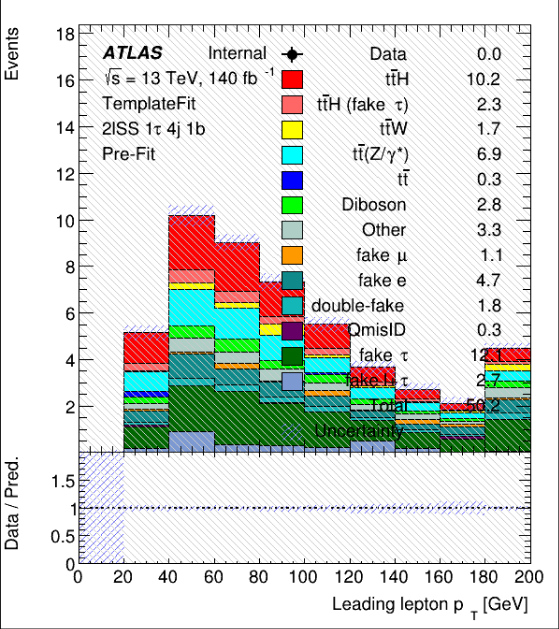
\includegraphics[width=\linewidth]{figures/plots/histograms/lep_Phi_1.png}
        \caption{Distribution of the azimuthal angle of the subleading lepton.}
        \label{fig:lep_Phi_1}
    \end{subfigure}

    \vspace{0.5cm}

    \begin{subfigure}{0.45\textwidth}
        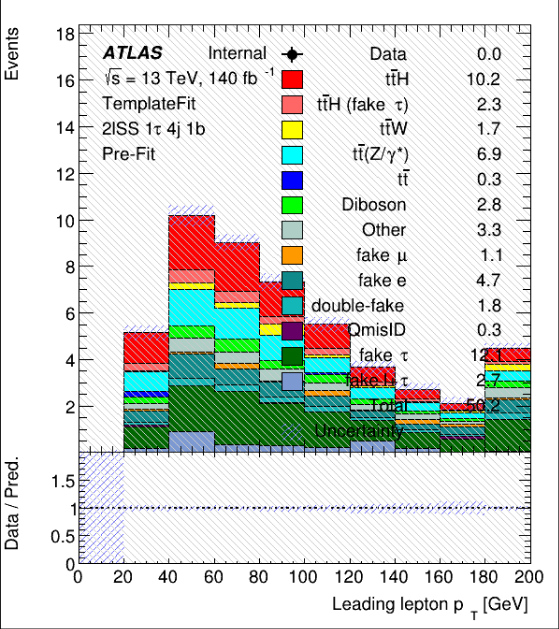
\includegraphics[width=\linewidth]{figures/plots/histograms/njets.png}
        \caption{Distribution of the number of jets.}
        \label{fig:njets}
    \end{subfigure}\hfill%
    \begin{subfigure}{0.45\textwidth}
        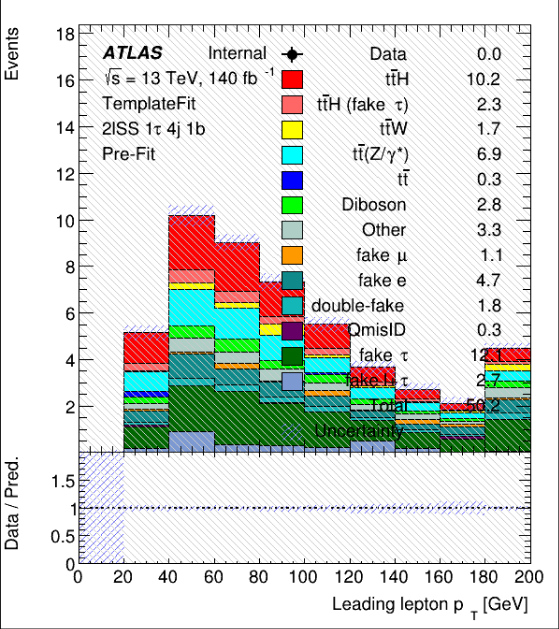
\includegraphics[width=\linewidth]{figures/plots/histograms/nbjets.png}
        \caption{Distribution of the number of $b$-jets.}
        \label{fig:nbjets}
    \end{subfigure}
    \caption{Distributions of the variables inside \gls{sr} (part 2)}
    \label{fig:distributions2}
\end{figure}

\begin{minipage}{0.45\textwidth}
    \centering
    \begin{tabular}{c|c|c|c|c}
        $t\bar{t}H$ & \textbf{v6} & \textbf{v8} &      &       \\
        \hline
        Weighted    & 1000        & 500         & -500 & -50\% \\
        Raw         & 1000        & 500         & -500 & -50\% \\
        \hline
    \end{tabular}
    \captionof{table}{Number of ttH events in the SR for v6 and v8.}
    \label{tab:ttH_event_numbers1}
\end{minipage}\hfill%
\begin{minipage}{0.45\textwidth}
    \centering
    \begin{tabular}{c|c|c|c|c}
        \gls{sr} & \textbf{v6} & \textbf{v8} &      &       \\
        \hline
        Weighted & 1000        & 500         & -500 & -50\% \\
        Raw      & 1000        & 500         & -500 & -50\% \\
        \hline
    \end{tabular}
    \captionof{table}{Number of all the events in the SR for v6 and v8.}
    \label{tab:ttH_event_numbers2}
\end{minipage}

\clearpage \subsection{Features used}

\subsubsection{\texttt{lep\_E\_X}} The energy of the Xth lepton.

\subsubsection{\texttt{DRjj\_lead}} $\Delta R$ between the two leading jets. $\Delta R$ is a distance metric in the
$\eta-\phi$ space frequently used in particle physics.

\subsubsection{\texttt{Ptll01}} The transverse momentum of the dilepton system made up of the two leading leptons.

\subsubsection{\texttt{lep\_nTrackParticles\_X}} The number of track particles associated with the Xth lepton.

\subsubsection{\texttt{custTrigMatch\_LooseID\_FCLooseIso\_DLT}} Custom trigger matching for loosely identified and loosely
isolated leptons, likely related to the dilepton trigger

\subsubsection{\texttt{Mll01}} The invariant mass of the two leading leptons.

\subsubsection{\texttt{Mlll012}} The invariant mass of the three leading leptons.

\subsubsection{\texttt{total\_charge}} The sum of the electric charges of the particles in the event.

\subsubsection{\texttt{HT}} The scalar sum of the transverse momenta of all jets in the event.

\subsubsection{\texttt{HT\_lep}} The scalar sum of the transverse momenta of all leptons in the event.

\subsubsection{\texttt{lep\_Eta\_X}} The pseudorapidity of the Xth lepton.

\subsubsection{\texttt{nTaus\_OR\_Pt25}} The number of overlapping-removed taus with a transverse momentum above 25 GeV.

\subsubsection{\texttt{nFwdJets\_OR}} The number of overlapping-removed forward jets.

\subsubsection{\texttt{MLepMet}} The invariant mass of a lepton and the missing transverse energy vector.

\subsubsection{\texttt{taus\_DL1r\_X}} The DL1r score for the Xth tau.

\subsubsection{\texttt{lep\_isolationLoose\_VarRad\_X}} Indicates whether a lepton (where X refers to the lepton index)
passes an isolation cut with a variable radius. Looser isolation cuts allow more nearby activity in the detector.

\subsubsection{\texttt{lep\_EtaBE2\_X}} The pseudorapidity of the Xth lepton in the second layer of the electromagnetic
calorimeter.

\subsubsection{\texttt{HT\_fwdJets}} The scalar sum of the transverse momenta of all forward jets in the event.

\subsubsection{\texttt{taus\_width\_X}} The width of the Xth tau.

\subsubsection{\texttt{nJets\_OR\_DL1r\_85}} Count of jets that pass overlap removal (OR) and are b-tagged according to the
DL1r algorithm at the 85\% working point.

\subsubsection{\texttt{lep\_nInnerPix\_X}} Number of hits in the inner pixel detector associated with the lepton, where X
refers to the lepton index.

\subsubsection{\texttt{met\_phi}} The azimuthal angle of the missing transverse energy in the event.

\subsubsection{\texttt{DeltaR\_max\_lep\_bjet77}} The maximum DeltaR value between a lepton and a b-tagged jet. The "77"
may refer to the working point of the b-tagging algorithm.

\subsubsection{\texttt{MbX}} Invariant mass associated with the leading b-jet in the event

\subsubsection{\texttt{lep\_RadiusCO\_X}} Possibly the radius of the cone used for isolation of the lepton, or
alternatively a parameter associated with the trajectory of the lepton.

\subsubsection{\texttt{lep\_Mtrktrk\_atConvV\_CO\_X}} The invariant mass of track pairs at the conversion vertex for lepton
X. This might be related to photon conversions into an electron-positron pair.

\subsubsection{\texttt{lep\_Z0SinTheta\_X}} The z0 impact parameter times the sine of the lepton's polar angle.

\subsubsection{\texttt{lep\_Pt\_X}} The transverse momentum of the Xth lepton.

\subsubsection{\texttt{mjjMax\_frwdJet}} The maximum invariant mass of a pair of forward jets.

\subsubsection{\texttt{dilep\_type}} The type of dilepton event (e.g., $ee$, $\mu e$, $\mu \mu$).

\subsubsection{\texttt{eta\_frwdjet}} The pseudorapidity of the forward jet.

\subsubsection{\texttt{Mlb}} Invariant mass of a lepton and a b-jet.

\subsubsection{\texttt{taus\_RNNJetScoreSigTrans\_X}} Transformed RNN-based score for tau lepton, possibly to better
separate signal from background.

\subsubsection{\texttt{minDeltaR\_LJ\_X}} The minimum $\Delta R$ distance between the Xth lepton and any jet in the event.

\subsubsection{\texttt{nTaus\_OR}} Number of tau leptons that pass overlap removal. Overlap removal is a step in particle
reconstruction where, for instance, an object identified as both a jet and a tau would be considered only as one or the
other.

\subsubsection{\texttt{DeltaR\_min\_lep\_jet}} The minimum $\Delta R$ distance between a lepton and a jet in the event.

\subsubsection{\texttt{lep\_sigd0PV\_X}} Significance of the transverse impact parameter (d0) of the lepton X with respect
to the primary vertex (PV). This is a common variable for distinguishing prompt particles produced in the primary
collision from secondary particles produced in a decay.

\subsubsection{\texttt{taus\_eta\_X}} The pseudorapidity of the Xth tau.

\subsubsection{\texttt{HT\_jets}} The scalar sum of the transverse momenta of all jets (not forward jets) in the event.

\subsubsection{\texttt{lep\_Phi\_X}} The azimuthal angle (in radians) of the Xth lepton.

\subsubsection{\texttt{bTagSF\_weight\_DL1r\_85}} A weight applied to events based on the scale factor for b-tagging using
the DL1r algorithm at an 85\% efficiency working point. This scale factor corrects the b-tagging efficiency in Monte
Carlo simulations to match that observed in real data.

\subsubsection{\texttt{lep\_chargeIDBDTResult\_recalc\_rel207\_tight\_X}} The outcome of a BDT-based charge identification
for a lepton, recalculated with some specific settings, and applying a 'tight' threshold.

\subsubsection{\texttt{taus\_phi\_X}} The azimuthal angle (in radians) of the Xth tau.

\subsubsection{\texttt{taus\_passJVT\_X}} A boolean flag indicating whether the Xth tau passes the jet vertex tightness
(JVT) requirement.

\subsubsection{\texttt{jets\_eta}} The pseudorapidity of the jets (array).

\subsubsection{\texttt{taus\_charge\_X}} The charge of the Xth tau.

\subsubsection{\texttt{passPLIVTight\_X}} Boolean flag indicating if a lepton with high transverse momentum passes the
"tight" criteria of the Prompt Lepton Veto (PLIV), a tool for identifying non-prompt light leptons.

\subsubsection{\texttt{lep\_Mtrktrk\_atPV\_CO\_X}} The invariant mass of track pairs at the primary vertex for lepton X.
This could be related to certain types of particle decays happening at the primary collision vertex.

\subsubsection{\texttt{taus\_JetRNNSigMedium\_X}} RNN-based score for tau lepton, used to distinguish tau leptons from
jets, with 'medium' selection criteria.

\subsubsection{\texttt{minOSMll}} The minimum invariant mass of oppositely-signed dilepton pairs.

\subsubsection{\texttt{lep\_ID\_X}} The identification number for the Xth lepton.

\subsubsection{\texttt{Mllll0123}} The invariant mass of the four leading leptons.

\subsubsection{\texttt{custTrigSF\_TightElMediumMuID\_FCLooseIso\_DLT}} Custom trigger scale factor, for events with a
tight electron and a medium muon, both of which are loosely isolated, likely related to the dilepton trigger (DLT).

\subsubsection{\texttt{best\_Z\_Mll}} The invariant mass of the dilepton system that is closest to the Z boson mass.

\subsubsection{\texttt{met\_met}} The missing transverse energy in the event.

\subsubsection{\texttt{MtLep1Met}} Transverse mass between the leading lepton and missing transverse energy. Transverse
mass is often used in searches for particles that decay to a lepton and a neutrino.

\subsubsection{\texttt{lep\_ambiguityType\_X}} Type of ambiguity for lepton identification, where X refers to the lepton
index. Ambiguity could arise from several factors, such as a single track matching with multiple reconstructed
particles.

\subsubsection{\texttt{jets\_phi}} The azimuthal angle (in radians) of the jets (array).

\subsubsection{\texttt{lep\_isMedium\_X}} Boolean flag indicating if a lepton passes the 'medium' selection criteria.

\subsubsection{\texttt{taus\_RNNJetScore\_X}} RNN-based score for tau lepton, used to distinguish tau leptons from jets.

\subsubsection{\texttt{MtLepMet}} The transverse mass of a lepton and the missing transverse energy vector.

\subsubsection{\texttt{DeltaR\_min\_lep\_jet\_fwd}} The minimum $\Delta R$ distance between a lepton and a forward jet in the event.

\subsubsection{\texttt{jets\_e}} The energy of the jets (array).

\subsubsection{\texttt{minOSSFMll}} The minimum invariant mass of oppositely-signed, same-flavor dilepton pairs.

\subsubsection{\texttt{nJets\_OR}} The number of overlapping-removed jets.

\subsubsection{\texttt{total\_leptons}} The total number of leptons in the event.

\subsubsection{\texttt{taus\_numTrack\_X}} The number of tracks associated with the Xth tau.

\subsubsection{\texttt{HT\_taus}} Scalar sum of the transverse momenta ($P_t$) of all tau leptons in the event.

\subsubsection{\texttt{taus\_passEleOLR\_X}} A boolean flag indicating whether the Xth tau passes the electron overlap
removal.

\subsubsection{\texttt{HT\_inclFwdJets}} The scalar sum of the transverse momenta of all jets, including forward jets, in
the event.

\subsubsection{\texttt{DRll01}} The $\Delta R$ distance between the two leading leptons.

\subsubsection{\texttt{taus\_JetRNNSigLoose\_X}} RNN-based score for tau lepton, used to distinguish tau leptons from
jets, with 'loose' selection criteria.

\subsubsection{\texttt{taus\_pt\_X}} The transverse momentum of the Xth tau.

\subsubsection{\texttt{bTagSF\_weight\_DL1r\_77}} A weight applied to events based on the scale factor for b-tagging using
the DL1r algorithm at an 77\% efficiency working point. This scale factor corrects the b-tagging efficiency in Monte
Carlo simulations to match that observed in real data.

\subsubsection{\texttt{flag\_JetCleaning\_LooseBad}} A flag variable indicating whether a jet passes a loose cleaning cut
to remove bad or noisy jets from the analysis.

\subsubsection{\texttt{taus\_fromPV\_X}} A boolean flag indicating whether the Xth tau comes from the primary vertex.

\subsubsection{\texttt{best\_Z\_other\_MtLepMet}} The transverse mass between the lepton and missing transverse energy for
the event that best reconstructs a Z boson using other criteria.

\subsubsection{\texttt{nJets\_OR\_DL1r\_77}} Count of jets that pass overlap removal (OR) and are b-tagged according to the
DL1r algorithm at the 77\% working point.

\subsubsection{\texttt{jets\_pt}} The transverse momentum of the jets (array).

\subsubsection{\texttt{lep\_isTightLH\_X}} Boolean flag indicating if a lepton passes the 'tight' Likelihood-based
identification criteria.

\subsubsection{\texttt{taus\_JetRNNSigTight\_X}} RNN-based score for tau lepton, used to distinguish tau leptons from
jets, with 'tight' selection criteria.

\subsubsection{\texttt{sumPsbtag}} The sum of b-tagging weights for jets in the event.

\subsubsection{\texttt{taus\_decayMode\_X}} The decay mode of the Xth tau.

\subsubsection{\texttt{dEta\_maxMjj\_frwdjet}} The maximum difference in pseudorapidity ($\eta$) between two forward jets.

\subsubsection{\texttt{max\_eta}} The maximum pseudorapidity among all particles in the event.

\subsubsection{\texttt{best\_Z\_other\_Mll}} The invariant mass of the dilepton system that is closest to the Z boson mass,
not considering the leading leptons.

\subsubsection{\texttt{taus\_passEleBDT\_X}} Flag indicating if a tau lepton passes the Electron Boosted Decision Tree
discriminator.

\begin{figure}[hbtp]
    \centering
    \includegraphics[width=\textwidth]{figures/ml/features/top20.pdf}
    \caption{Feature importance for the top 20 most important features. Feature importance was calculated using the
        \gls{ig} method \cite{ig}.}
    \label{fig:feature_importance}
\end{figure}

\clearpage


\subsection{Regions in Particle Physics}

In particle physics, especially in high energy experiments such as those conducted at the LHC, the parameter space is
vast. Identifying signals from noise or background events becomes a challenging task. To tackle this challenge, we
divide the parameter space into different regions, each serving a specific purpose. These regions include the \gls{sr},
\gls{cr}, and \gls{vr}.

\begin{itemize}
    \item \textbf{\gls{sr}} is where we expect the events of interest, the
          signal, to be most prevalent. It is defined by certain selection criteria that maximize the signal's prominence against
          the background. In our case, the signal refers to the \tth events.

    \item \textbf{\gls{cr}} is where we estimate the amount of background contamination
          present in the \gls{sr}. The \gls{cr} is characterized by negligible signal but a significant amount of background
          events, similar to what we expect in the \gls{sr}. By studying the \gls{cr}, we can understand and model the background in the \gls{sr}.

    \item \textbf{\gls{vr}} is used to test the reliability of our model predictions
          and the \gls{mc} simulations. The VR is typically chosen where neither the signal nor the background is expected to
          be particularly high or low. Any significant deviation of the observed data from our model predictions in the VR may
          indicate the presence of a new physics process or systematic errors in our model or simulation.
\end{itemize}

These regions are not arbitrarily defined but are carefully chosen based on detailed knowledge of the physics processes
involved and the detector's characteristics. They provide a robust framework for analyzing the data from high-energy
physics experiments and are crucial in our search for the \tth process events.

\subsection{\lss channel}
\label{sec:lss}

% ttH
\begin{figure}[htb]
    \centering
    \begin{tikzpicture}
        \begin{feynhand}
            \vertex[dot] (c) at (0,0) {};
            \vertex[dot] (h) at (2,0) {};
            \vertex[dot] (g1) at (-1.5, 1) {};
            \vertex[dot] (g11) at (-3.5,2);
            \vertex[dot] (t) at (2,2);
            \vertex[dot] (g2) at (-1.5, -1) {};
            \vertex[dot] (g21) at (-3.5,-2);
            \vertex[dot] (tbar) at (2,-2);

            % Production of H
            \propag [scalar] (c) to [edge label=\(H\)] (h);
            \propag [anti fermion] (g1) to [edge label=\(\bar{t}\)] (c);
            \propag [fermion] (g2) to [edge label=\(t\)] (c);
            % Production of t
            \propag [fermion] (g1) to [edge label=\(t\)] (t);
            % Production of tbar
            \propag [anti fermion] (g2) to [edge label=\(\bar{t}\)] (tbar);
            % Gluon splitting
            \propag [gluon] (g11) to [edge label=\(g\)] (g1);
            \propag [gluon] (g21) to [edge label=\(g\)] (g2);
        \end{feynhand}
    \end{tikzpicture}
    \caption{Feynman diagram of the \lss process.}
    \label{fig:2lss1tau}
\end{figure}

The work at CERN is often divided into different channels, with each channel focusing on a specific final state of
interest. These channels are orthogonal, meaning that each event can only belong to one channel, preventing any overlap
in the analysis.

One such channel, and the main focus of this thesis, is the two-lepton same-sign plus one tau (\lss) channel. This
specific final state arises from the decay of a top-antitop-Higgs (\tth) system, where one top quark decays to a W boson
and a b quark, with the W boson further decaying to a lepton and a neutrino. The other top quark also decays to a W
boson and a b quark, but in this case, the W boson decays into a pair of quarks. Lastly, the Higgs boson decays to a
pair of tau leptons, where one tau lepton decays into another lepton and two neutrinos, while the other tau lepton
decays to a pair of quarks and a neutrino. This complex series of decays results in a final state consisting of two
same-sign leptons and a hadronically decaying tau lepton, hence the name \lss channel (as shown in \autoref{fig:2lss1tau}).

The branching ratios for these decays are as follows:

\begin{align*}
    \text{Higgs boson to a pair of tau leptons: }\mathcal{B}(H \rightarrow \tau\tau)  & = 6.25\% \\
    \text{tau lepton to a W boson and a neutrino: }\mathcal{B}(\tau \rightarrow W\nu) & = 100\%  \\
    \text{top quark to a W boson and a b quark: }\mathcal{B}(t \rightarrow Wb)        & = 100\%  \\
    \text{W boson to a lepton and a neutrino: }\mathcal{B}(W \rightarrow l\nu)        & = 10\%   \\
    \text{W boson to a pair of quarks: }\mathcal{B}(W \rightarrow qq)                 & = 70\%
\end{align*}

Given that the theoretical cross-section for the \tth process is 500 fb and the luminosity is 140 fb$^{-1}$, the total
number of expected \tth events is approximately 70,000. When accounting for the aforementioned branching ratios, the
expected number of \tth events in the \lss final state is reduced to:

\begin{align*}
    N_{\text{\tth, \lss}} & = \sigma_{\text{\tth}} \cdot \mathcal{L} \cdot \mathcal{B}(H \rightarrow \tau\tau) \cdot \mathcal{B}(\tau \rightarrow W\nu) \cdot \mathcal{B}(t \rightarrow Wb) \cdot \mathcal{B}(W \rightarrow l\nu) \cdot \mathcal{B}(W \rightarrow qq) \\
                          & = 500 \text{ fb} \cdot 140 \text{ fb}^{-1} \cdot 6.25\% \cdot 100\% \cdot 100\% \cdot 10\% \cdot 70\% \approx 3.15
\end{align*}

\todo{Fix the above calculations, it's not correct}

% It should be noted, however, that this is a simplified calculation and does not consider various factors such as
% detector efficiencies and background events. Nevertheless, it provides a good estimate of the scale of the challenge we
% face in detecting the \tth process in the \lss channel.

As we apply the selection criteria to the data, we drop from about 8.9M to just 32K raw events. For the \tth, this
corresponds to 0.8M $\rightarrow$ 15K raw events. In terms of weighted events the transition is from 46K $\rightarrow$
32.72 weighted events across all the processes, and 523.42 $\rightarrow$ 12.22 weighted events for the \tth. The details
for all processes are shown on the \autoref{tab:class_distributions}.

\todo{highlight the numbers above}

\begin{figure}[htb]
    \centering
    \begin{tabular}{l|rr|rr}
Process & SR (Raw) & SR (Weighted) & ALL (Raw) & ALL (Weighted) \\
\hline
\tth & 15293 & 12.22 & 834970 & 523.42 \\
\ttw & 1479 & 5.49 & 581089 & 1680.34 \\
\ttwew & 74 & 0.59 & 15314 & 122.36 \\
\ttz & 9612 & 7.78 & 1750978 & 1550.66 \\
\ttbar & 3 & 0.33 & 299808 & 33487.35 \\
$VV$ & 1433 & 2.55 & 3829589 & 7046.18 \\
$tZ$ & 32 & 0.29 & 40946 & 378.09 \\
$WtZ$ & 209 & 1.20 & 45931 & 248.63 \\
$tW$ & 0 & 0.00 & 4493 & 413.89 \\
$t\bar{t}t$ & 449 & 0.16 & 22980 & 8.08 \\
$t\bar{t}t\bar{t}$ & 482 & 0.97 & 22746 & 45.27 \\
$ggVV$ & 38 & 0.01 & 792331 & 354.08 \\
$VVV$ & 20 & 0.02 & 151324 & 60.93 \\
$VH$ & 0 & 0.00 & 255 & 102.55 \\
$WttW$ & 94 & 0.81 & 5944 & 50.56 \\
$tHjb$ & 3058 & 0.14 & 445666 & 21.41 \\
$tWH$ & 492 & 0.18 & 30587 & 15.95 \\
\hline
Total & 32768 & 32.72 & 8874951 & 46109.77 \\
\end{tabular}

    \captionof{table}{Comparison of the number of events before and after applying the selection criteria. For each
        process, we show the number of raw events and the number of weighted events.}
    \label{tab:class_distributions}
\end{figure}


The figures \autoref{fig:lep_pt_0} and \autoref{fig:lep_pt_1} show the distributions of the leading and
subleading leptons' transverse momenta inside inside the \gls{sr}. These types of plots are one of the most common
plots generated by the \trex\footnote{\trex is a framework for binned template profile likelihood fits heavily used at
    CERN. The documentation can be found at \url{https://trexfitter-docs.web.cern.ch/trexfitter-docs/}. The code can be
    found at \url{https://gitlab.cern.ch/TRExStats/TRExFitter}} software. These plots are often used to check the well
modelling of the variables. It is essential to make sure that the variables are well
modelled - events generated by the \gls{mc} agrees with the real data. Otherwise we can be training on the wrong data
and our classifier will not generalize well when it comes to the real data. More plots are presented in the
\appref{appendix:yields}.


\captionsetup[subfigure]{justification=centering}
\begin{figure}[htb]
    \centering
    \begin{subfigure}{0.45\textwidth}
        \includegraphics[width=\linewidth]{figures/yields/lep-pt-0.pdf}
        \caption{Distribution of the transverse momentum of the leading lepton.}
        \label{fig:lep_pt_0}
    \end{subfigure}\hfill%
    \begin{subfigure}{0.45\textwidth}
        \includegraphics[width=\linewidth]{figures/yields/lep-pt-1.pdf}
        \caption{Distribution of the transverse momentum of the subleading lepton.}
        \label{fig:lep_pt_1}
    \end{subfigure}
    \caption{Distributions of the transverse momentum of the leading and subleading leptons. The areas are crossed out
        because the events in these regions are blinded.}
\end{figure}

One might wonder why the plots are crossed out in some regions. This is because the events in these regions are blinded.
Blinding refers to hiding the data points in the bin if the relation of teh signal to background is larger than some
threshold. A threshold of $0.15$ is a common threshold to apply and that is what we have used throughout the thesis.
The reasoning behind the blinding is \todo{???}.

